\documentclass{../industrial-development}

    \graphicspath{{8-9-project-managment/}}
    \usepackage{multirow}
    \newcommand{\sz}{\footnotesize}
    \newcommand{\zz}{\phantom{0}}
    
    \title{Управление программными проектами}
    \author{Никитин Евгений Сергеевич,\\Быков Михаил Дмитриевич,\\ИВТ-21 МО}
    \date{}
    
    \begin{document}
    
    \begin{frame}
      \titlepage
    \end{frame}

    \section{Программные проекты}

    \subsection{Основные понятия}

    \begin{frame} \frametitle{Продукт}
        \begin{definition}
            Продукт - ???
        \end{definition}
        \medskip
        Важное замечание о продукте.
    \end{frame}

    \begin{frame} \frametitle{Проект}
        \begin{definition}
            Проект - временное предприятие, предназначенное для~создания уникальных продуктов, услуг или результатов
        \end{definition}
        \medskip
        В проекте должны быть определены:
        \begin{itemize}
            \item Цели и результаты (область охвата)
            \item Уровень качества
            \item Этапы и сроки выполнения работ
            \item Бюджет
        \end{itemize}
    \end{frame}
    \lecturenotes
    Заглушка
    
    \begin{frame} \frametitle{Треугольник проекта}
        % \centerline{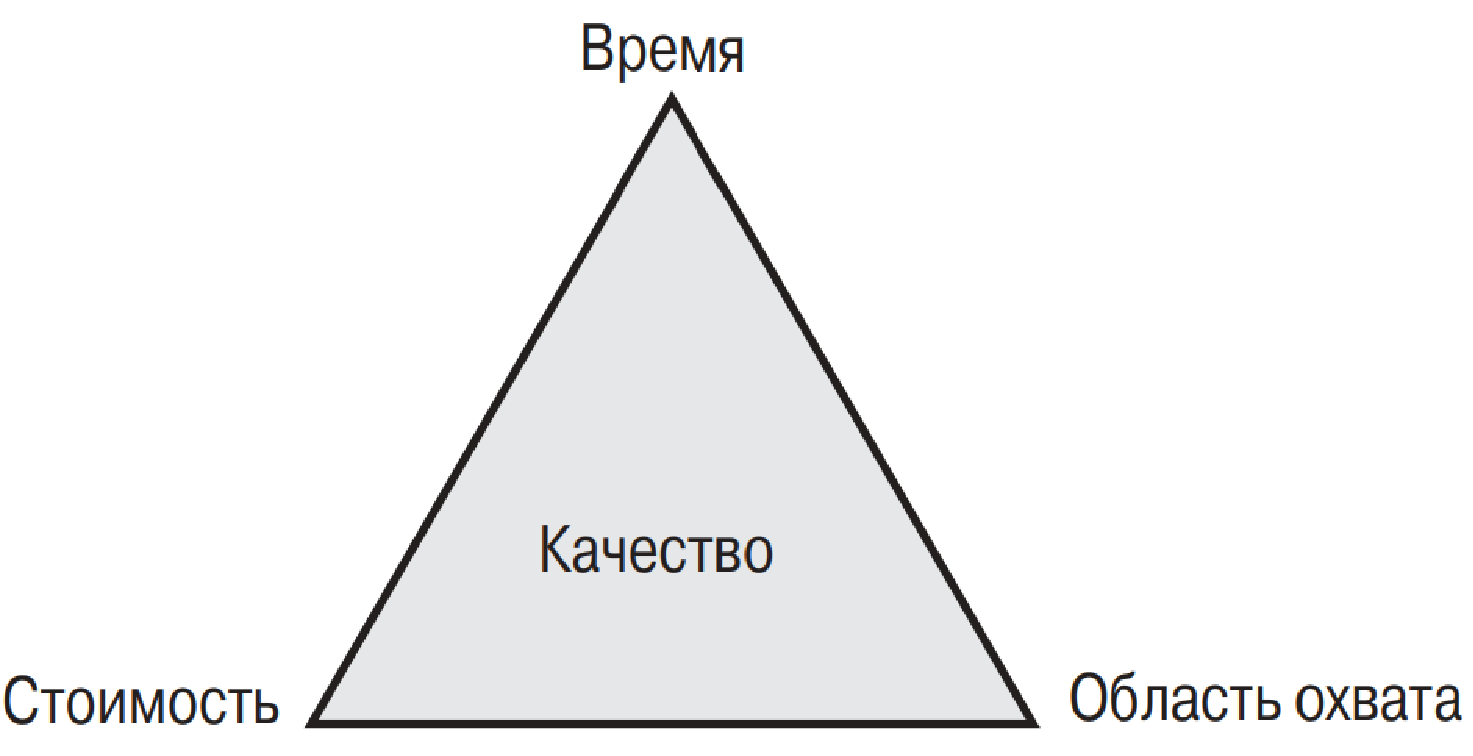
\includegraphics[width=0.5\textwidth]{trinagle.pdf}} %
        \begin{block}{Идеальный проект}
            \begin{itemize}
                \item Соблюдены сроки выполнения
                \item Результат соответствует целям
                \item Затраты в пределах бюджета
            \end{itemize}
        \end{block}
        \medskip
        Не стоит забывать про \alert{качество}!
    \end{frame}
    \lecturenotes
    Заглушка

    \begin{frame} \frametitle{Процессы проекта}
        \begin{definition}
            Процессы проекта - ?
        \end{definition}
        \medskip
        Этапы:
        \begin{itemize}
            \item Почему - обоснование проекта
            \item Что - техническое задание
            \item Как - модель жизненного цикла
            \item Выполнение - выполнение жизненного цикла
            \item Сделано - анализ эффективности выполнения
        \end{itemize}
    \end{frame}
    \lecturenotes
    Заглушка

    \begin{frame} \frametitle{Процессы продукта и проекта}
        \begin{block}{Важно}
            \begin{itemize}
            \item Процессы \alert{продукта} описывают создание программного продукта
            \item Процессы \alert{проекта} описывают, как будет выполняться разработка
            \end{itemize}
        \end{block}
    \end{frame}
    \lecturenotes
    Заглушка

    \subsection{Процессы проекта: Почему, Что и Как}

    \begin{frame} \frametitle{Процессы проекта: Почему, Что и Как}
        Общий текст про обоснование, тз и жизненный цикл
    \end{frame}
    \lecturenotes
    Заглушка
    
    \begin{frame} \frametitle{Почему: обоснование проекта}
        Текст про обоснование проекта.
    \end{frame}
    \lecturenotes
    Заглушка

    \begin{frame} \frametitle{Что: техническое задание}
        \begin{definition}
            Техническое задание - это документ, формально определяющий существование проекта
        \end{definition}
        \begin{block}{Перечень вопросов по техническому заданию}
            \begin{itemize}
            \item Цели проекта
            \item Промежуточные результаты работы
            \item Контрольные точки
            \item Технические требования
            \item Ограничения и исключения
            \item Проверка выполнения работы совместно с клиентом
            \end{itemize}
        \end{block}
    \end{frame}
    \lecturenotes
    Заглушка

    \begin{frame} \frametitle{Цель проекта}
        \begin{block}{}
            Цель должна быть четко определена!
        \end{block}
        \begin{block}{}
            Завершение проекта - это одна из главных целей
        \end{block}
        \begin{block}{}
            Основная цель должна быть описана сжато, но понятно для всех участников
        \end{block}
    \end{frame}
    \lecturenotes
    Заглушка

    \begin{frame} \frametitle{Ограничения и исключения}
        \begin{definition}
            Рабочая область - это рабочий план, включающий описание требований
        \end{definition}
        \begin{block}{}
            Необходимо точно определить границы рабочей области проекта
        \end{block}
    \end{frame}
    \lecturenotes
    Заглушка
    
    \begin{frame} \frametitle{Как: жизненный цикл проекта}
        \centerline{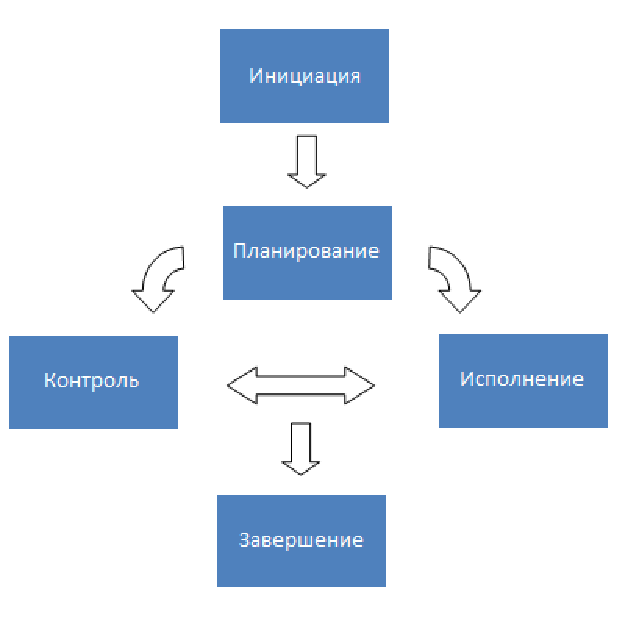
\includegraphics[width=0.7\textwidth]{manageproject.pdf}}
    \end{frame}
    \lecturenotes
    Заглушка

    \subsection{Жизненный цикл проекта: шаги к успеху}
    
    \begin{frame} \frametitle{Инициация}
        \begin{block}{Назначение}
            Определяется суть проекта, его цель, заинтересованные в~нём лица. Чем меньше проект, тем проще эта стадия проходит
        \end{block}
        Этапы:
        \begin{itemize}
            \item Описание проблемы
            \item Определение требований
        \end{itemize}
    \end{frame}
    \lecturenotes
    Заглушка
    
    \begin{frame} \frametitle{Планирование}
        \begin{block}{Назначение}
            Составляется список задач и мероприятий, которые должны быть выполнены в рамках проекта. Также указывается взаимосвязь между задачами и требующиеся ресурсы
        \end{block}
        Параллельно планированию обычно проводится оценка рисков и разрабатывается стратегия для их~предупреждения
    \end{frame}
    \lecturenotes
    Заглушка

    \begin{frame} \frametitle{Исполнение и контроль}
        Исполнение и контроль проекта происходит циклами:
        \begin{itemize}
            \item Создание плана
            \item Реализация его части
            \item Контроль исполнения
            \item Внесение изменений в план
        \end{itemize}
    \end{frame}
    \lecturenotes
    Заглушка

    \begin{frame} \frametitle{Завершение}
        Текст про особенности завершения.
    \end{frame}
    \lecturenotes
    Заглушка

    \section{Управление проектами}

    \subsection{Зачем управлять проектами}

    \begin{frame} \frametitle{Управление проектами}
        \begin{definition}
            Управление проектами - область деятельности, в ходе которой определяются и достигаются четкие цели проекта при балансировании между объёмом работ, ресурсами, временем, качеством и рисками
        \end{definition}
    \end{frame}
    \lecturenotes
    Заглушка

    \begin{frame} \frametitle{Задачи управления проектами}
        Задачами управления проекта являются:
        \begin{itemize}
            \item Определение цели проекта
            \item Создание структуры проекта
            \item Определение необходимых объемов и источников финансирования
            \item Подбор команды исполнителей
            \item Определение сроков выполнения проекта
            \item Планирование и учет рисков
            \item Обеспечение контроля за ходом выполнения проекта
        \end{itemize}
    \end{frame}
    \lecturenotes
    Заглушка

    \begin{frame} \frametitle{Параметры управления проектами}
        % Очень много пунктов. Надо ли оно вообще? Почти идентично задачам
        Параметрами управления проектами являются:
        \begin{itemize}
            \item Сроки
            \item Объём проекта
            \item Объём работы
            \item Ценность проекта для потребителя
            \item Техническая и технологическая сложность
            \item Внешнее качество проекта
            \item Внутреннее качество проекта
            \item Риски
            \item Психологическое состояние команды
        \end{itemize}
    \end{frame}
    \lecturenotes
    Заглушка

    \begin{frame} \frametitle{Процессы управления программными проектами}
        Основные процессы управления проектом:
        \begin{itemize}
            \item Управление задачами
            \item Управление сроками
            \item Управление человеческими ресурсами
            \item Управление качеством
            \item Управление рисками
        \end{itemize}
    \end{frame}
    \lecturenotes
    Заглушка

    \subsection{Основные процессы управления проектами}

    \begin{frame} \frametitle{Управление задачами}
        \begin{block}{Назначение}
            Оценка объёма работы и распределение задач между сотрудниками
        \end{block}
        Основной инструмент - системы контроля задач.
    \end{frame}
    \lecturenotes
    Заглушка

    \begin{frame} \frametitle{Система контроля задач}
        \centerline{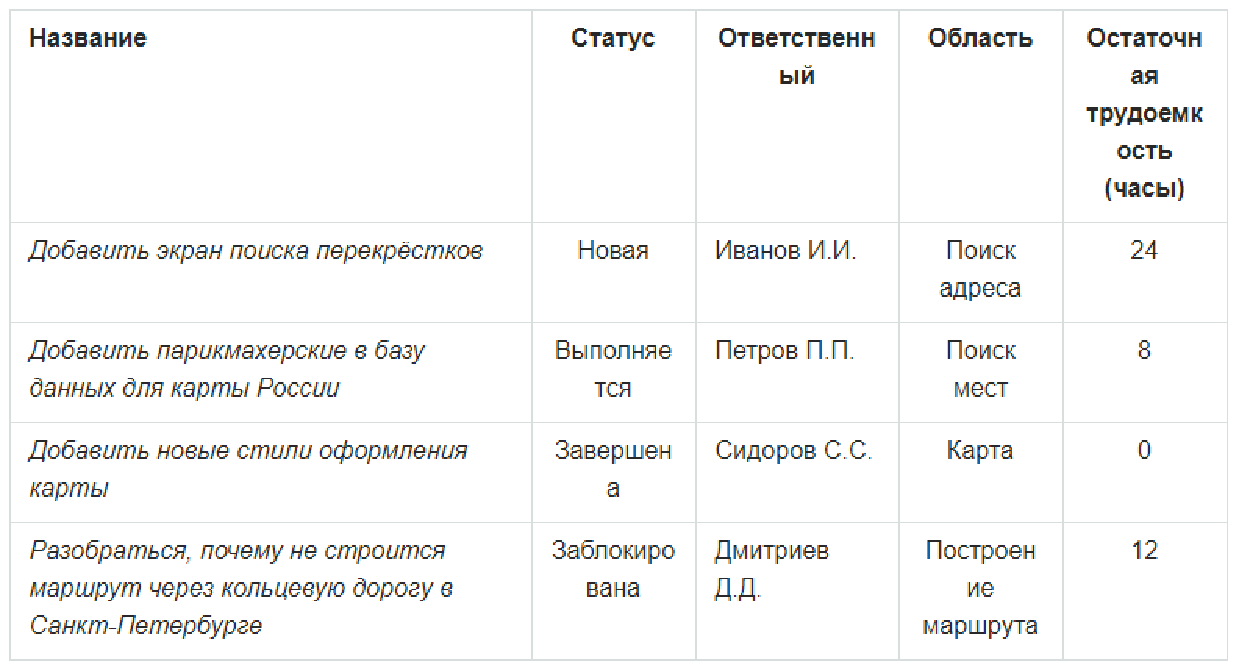
\includegraphics[width=1\textwidth]{gpstable.pdf}}
    \end{frame}
    \lecturenotes
    Заглушка

    \begin{frame} \frametitle{Система контроля задач}
        \centerline{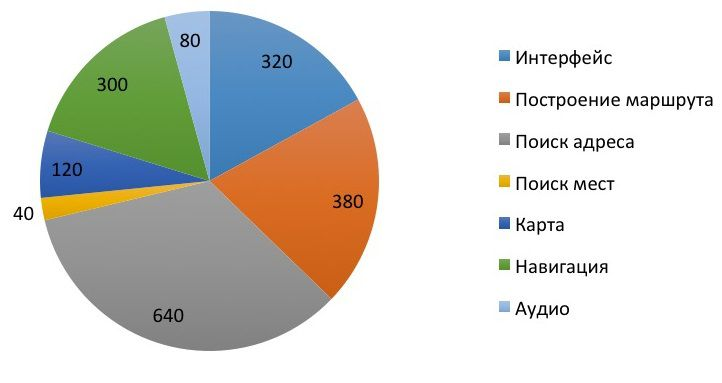
\includegraphics[width=1\textwidth]{circle.pdf}}
    \end{frame}
    \lecturenotes
    Заглушка
    
    \begin{frame} \frametitle{Система контроля задач}
        Цели системы контроля задач:
        \begin{itemize}
            \item Оценить и зафиксировать объём работы
            \item Распределить задачи между исполнителями
            \item Найти зависимости между различными задачами
            \item Определить, какие задачи заблокированы по тем или~иным причинам
        \end{itemize}
    \end{frame}
    \lecturenotes
    Заглушка

    \begin{frame} \frametitle{Использование системы контроля~задач}
        \begin{block}{}
            Первоначально задачи вносятся в систему контроля задач на этапе планирования проекта
        \end{block}
        Популярные системы контроля задач:
        \begin{itemize}
            \item Электронные таблицы Excel или Google Docs
            \item Redmine
            \item Jira
            \item BugZilla
            \item DropTask
            \item Hansoft
        \end{itemize}
    \end{frame}
    \lecturenotes
    Заглушка

    \begin{frame} \frametitle{Идентификация задач}
        \begin{block}{}
            Источником набора задач может быть личный опыт, опыт компании или данные об аналогичных проектах
        \end{block}
        \begin{block}{}
            Организации SEI, ISO и IEEE выложили в открытый доступ модели жизненного цикла, описания задач, которые выполняются на фазах цикла
        \end{block}
    \end{frame}
    \lecturenotes
    Заглушка
    
    \begin{frame} \frametitle{Декомпозиция задач}
        \begin{block}{}
            Задачи разбиваются на подзадачи непосредственно в процессе разработки, вместе с уточнением требований к проекту и обнаружением особенностей продукта или средств разработки
        \end{block}
    \end{frame}
    
    \lecturenotes
    Заглушка
    
    \begin{frame} \frametitle{Управление сроками}
        \begin{block}{Назначение}
            Оценка и контроль сроков реализации проекта
        \end{block}
        Цели управления сроками:
        \begin{itemize}
            \item Оценить текущий остаточный объём работы
            \item Определить величину отставания от плана
            \item Оценить прогресс каждого сотрудника и всей команды
        \end{itemize}
    \end{frame}
    \lecturenotes
    Заглушка

    \begin{frame} \frametitle{Методы распределения временных ресурсов}
        \begin{itemize}
            \item Календарный план
            \item Сетевое планирование
        \end{itemize}
    \end{frame}
    
    \begin{frame} \frametitle{Достоинства и недостатки календарного плана}
        \begin{block}{Достоинства}
            \begin{itemize}
                \item Легко расширить план новыми рубриками, т.е. строками таблицы
                \item План нагляден
            \end{itemize}
        \end{block}
        \begin{block}{Недостатки}
            \begin{itemize}
                \item Слишком быстро разрастается
                \item Не учитывает загруженность работников
                \item Не подходит для описания параллельных работ
            \end{itemize}
        \end{block}
    \end{frame}
  
    \begin{frame} \frametitle{Календарный план}
        \begin{definition}
            Календарный план "--- это последовательность работ проекта, разбитая по времени на этапы
        \end{definition}
        \begin{table}
            \caption{Пример таблицы с календарным планом}
            \center
            \begin{tabular}{ccccc}
                \hline
                \sz Наименование & \multicolumn{2}{c}{\sz Сроки выполнения\phantom{000}} & \sz Ответственные & \sz Ресурсы \\
                \sz работ & \sz план & \sz факт & \sz исполнители &  \\
                \hline
                1 & 2 & 3 & 4 & 5 \\
                \hline
            \end{tabular}
        \end{table}
    \end{frame}

    \begin{frame} \frametitle{Сетевое планирование}
        \begin{block}{Графы сетевого планирования}
            \begin{itemize}
                \item Графы, ориентированные на события
                \item Графы зависимостей работ
            \end{itemize}
        \end{block}
    \end{frame}

    \begin{frame} \frametitle{Диаграмма сгорания задач}
        Прогресс работы сотрудника (реальный и~прогнозируемый):
        \centerline{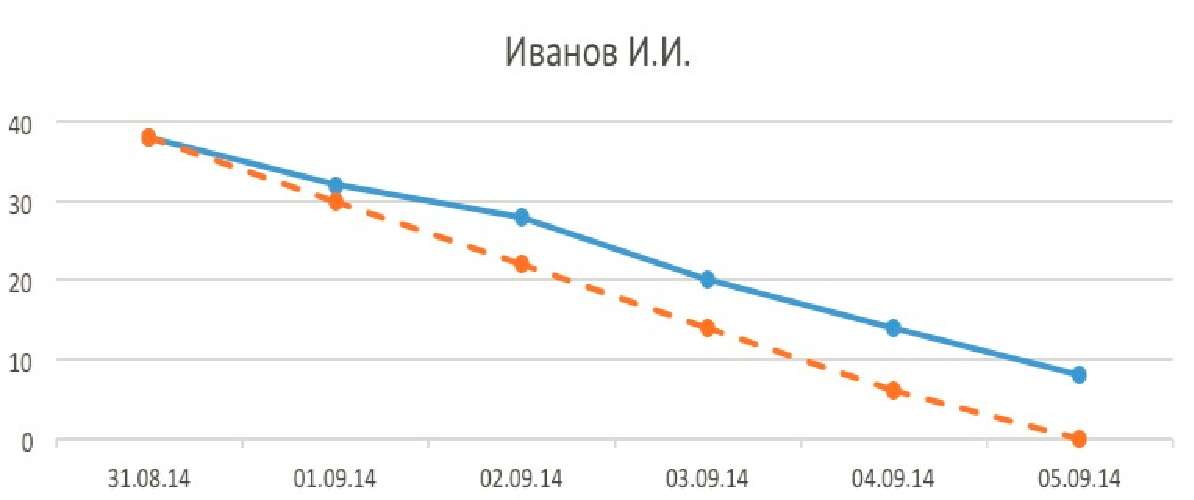
\includegraphics[width=1\textwidth]{ivanov.pdf}}
    \end{frame}
    
    \begin{frame} \frametitle{Диаграмма Гантта}
        \centerline{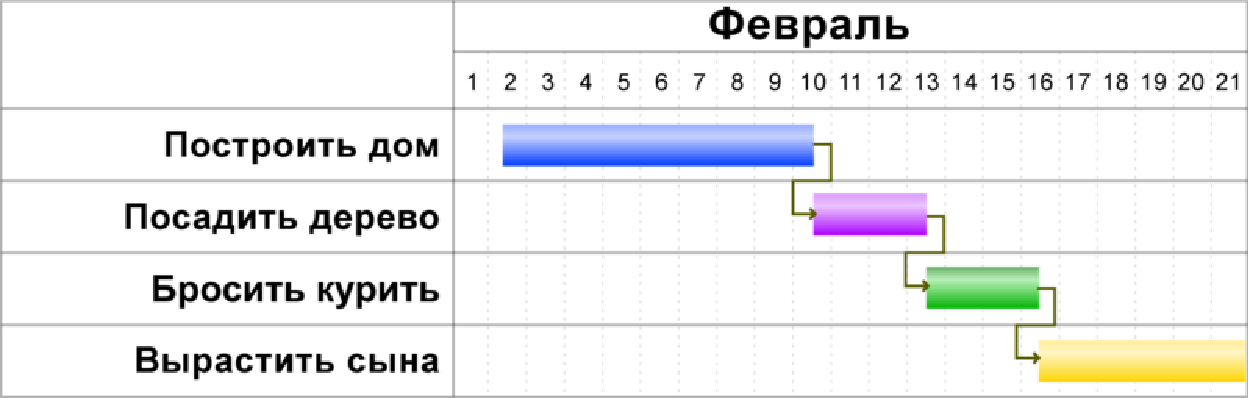
\includegraphics[width=1\textwidth]{gantt.pdf}}
    \end{frame}
    
    \begin{frame} \frametitle{Управление человеческими ресурсами}
        \begin{block}{Назначение}
            Наиболее эффективное использование человеческих ресурсов, вовлеченных в проект
        \end{block}
        Здесь что-то ещё написать
    \end{frame}
    \lecturenotes
    Заглушка

    \begin{frame} \frametitle{Кадровые ресурсы}    
        \begin{block}{Ключевые роли}
            \begin{itemize}
                \item Архитектор проекта
                \item Проектировщики подсистем
                \item Руководители команд разработки подсистем
                \item Специалист по пользовательскому интерфейсу
                \item Эксперт предметной области
            \end{itemize}
        \end{block}
    \end{frame}

    \begin{frame} \frametitle{Операционная бригада по Миллзу}
        \begin{itemize}
         \item Хирург "--- главный программист
         \item Второй пилот "--- проектировщик и программист
         \item Администратор
         \item Редактор документации
         \item Два секретаря
         \item Делопроизводитель
         \item Инструментальщик "--- программист, пишущий внутренние программы
         \item Отладчик "--- тестировщик
         \item Языковед "--- специалист по языку программирования
        \end{itemize}
    \end{frame}

    \begin{frame} \frametitle{Особенности организации работы больших команд}
        \begin{itemize}
            \item Современное проектирование как междисциплинарное согласование
            \item Наличие системного архитектора
            \item Коллективное определение потребностей
        \end{itemize}
    \end{frame}

    \begin{frame} \frametitle{Управление качеством продукта}
        \begin{block}{Назначение}
            Обеспечение надлежащего качества продукта
        \end{block}
        Цели
        \begin{itemize}
            \item Оценка сложности проекта
            \item Оценка ресурсов, необходимых на доводку качества
        \end{itemize}
    \end{frame}
    \lecturenotes
    Заглушка

    \begin{frame} \frametitle{Управление качеством продукта}
        Прогноз количества дефектов для мобильной навигационной системы GPS:
        \centerline{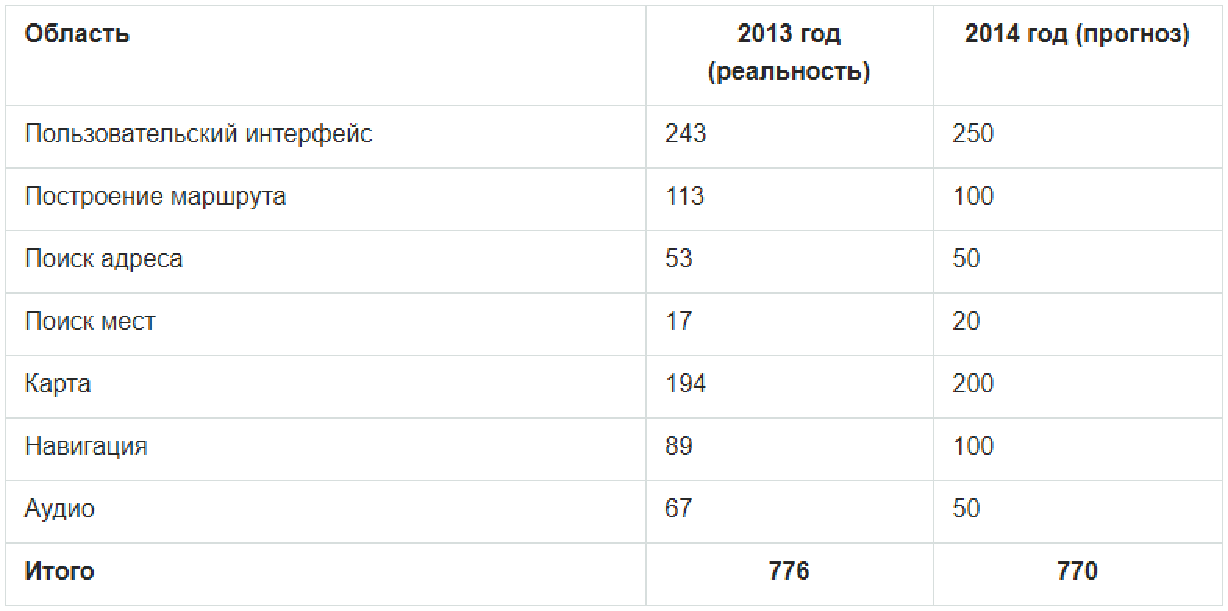
\includegraphics[width=1\textwidth]{gpstable1.pdf}}
    \end{frame}

    \begin{frame} \frametitle{Управление рисками}
        \begin{block}{Назначение}
            Предусмотреть риски, которые могут осложнить или сорвать проект, разработать план действий на случай срабатывания риска для нейтрализации его последствий
        \end{block}
        Цели:
        \begin{itemize}
            \item Описать выявленные риски
            \item Оценить важность каждого риска и вероятность его срабатывания
            \item Предложить план действия на случай того, если риск сработает
            \item Распределить риски между ответственными за их~устранение
        \end{itemize}
    \end{frame}
    \lecturenotes
    Заглушка

    \begin{frame} \frametitle{Оценка рисков}
        \begin{itemize}
            \item Идентификация рисков
            \item Анализ рисков
            \item Распределение приоритетов
        \end{itemize}
    \end{frame}
    
    \begin{frame} \frametitle{Оценка размеров и вероятностей потерь}
        \begin{block}{Оценка размеров}
            Для оценки сложной потери разбейте её на подзадачи и оценивайте их отдельно, затем объединяйте результат
        \end{block}
        
        \begin{block}{Методы оценки вероятности, уменьшающие её субъективность}
            \begin{itemize}
                \item Оценка специалистом
                \item Групповое обсуждение (метод Дельфи)
            \end{itemize}
        \end{block}
    \end{frame}

    \begin{frame} \frametitle{Оценка приоритетов рисков}
        \begin{block}{}
            Первый шаг - вычисление степени риска как произведения его вероятности на размер
        \end{block}
        
        \begin{block}{}
            Распределение и перераспределение приоритетов рисков всегда является субъективным
        \end{block}
        
        \begin{block}{}
            Не нужно тратить время на риски с низкой степенью
        \end{block}
    \end{frame}
    
    \begin{frame} \frametitle{Контроль рисков}
        \begin{itemize}
            \item Планирование управления рисками
            \item Разрешение рисков
            \item Мониторинг рисков
        \end{itemize}
    \end{frame}
    
    \begin{frame} \frametitle{Преодоление рисков}
        \begin{itemize}
         \item Исключение риска
         \item Уменьшение риск 
         \item Предупреждение ущерба от риска
         \item Планирование действий в непредвиденных ситуациях
        \end{itemize}
    \end{frame}

    \section{Мониторинг и коррекция процессов. Отчетность}

    \begin{frame} \frametitle{-}
        Далее идут слайды про мониторинг (в т.ч. отчетность) и коррекцию
    \end{frame}
    
    \end{document}

    %%% Local Variables: 
    %%% mode: TeX-pdf
    %%% TeX-master: t
    %%% End: 
